\section{Quantum Computation}

\subsection{Introduction to Qubits}

Classically, information is encoded as a binary string of 0s and 1s.

\begin{itemize}
    \itemsep 2pt
    \item 0 $\rightarrow$ 0000
    \item 1 $\rightarrow$ 0001
    \item 2 $\rightarrow$ 0010
    \item 3 $\rightarrow$ 0011
    \item 4 $\rightarrow$ 0100
    \item \dots
\end{itemize}

Meaning that, given $n$ bits, we can store $2^n$ possible binary strings.

In quantum computing, the $\ket 0$ and $\ket 1$ states form the computational basis.

\begin{equation*}
    \ket 0 = \begin{pmatrix} 1 \\ 0 \end{pmatrix} \qquad\qquad
    \ket 1 = \begin{pmatrix} 0 \\ 1 \end{pmatrix} \qquad
\end{equation*}

They are vectors in a two-dimensional complex Hilbert space $\mathbb{C}^2$, encoding information much in the same way that the classical computational basis does.

The $\ket 0$ and $\ket 1$ states can be represented on Bloch spheres.

\begin{figure}[H]
\centering
    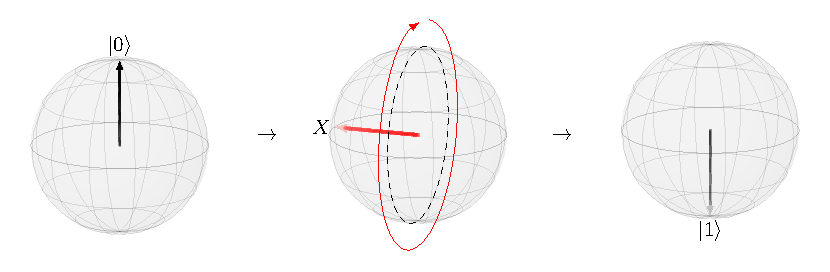
\includegraphics{blochspheres/zero_one}
    \caption{Bloch sphere representation of $\ket 0$ and $\ket 1$.}
\end{figure}

We can choose any pair of orthonormal states to form our computational basis.

\begin{equation*}
\begin{gathered}
    \ket + = \frac{1}{\sqrt{2}} (\ket 0 + \ket 1) \qquad\qquad
    \ket - = \frac{1}{\sqrt{2}} (\ket 0 - \ket 1)
\end{gathered}
\end{equation*}

\begin{figure}
\centering
\begin{blochsphere}[radius=1.5 cm,tilt=15,rotation=-20,opacity=0.05]
    \drawBallGrid[style={draw,opacity=0.1}]{30}{30}
    \drawStatePolar{zero}{0}{0}
    \labelPolar{zero}{0}{0};
    \node[above] at (zero) {{$\ket 0$}};
\end{blochsphere}
\end{figure}

Or equivalently, the two orthonormal $\ket R$ and $\ket L$ basis states.

\begin{equation*}
\begin{gathered}
    \ket R = \frac{1}{\sqrt{2}} (\ket 0 + i\ket 1) \qquad\qquad
    \ket L = \frac{1}{\sqrt{2}} (\ket 0 - i\ket 1)
\end{gathered}
\end{equation*}

More generally, any qubit $\ket\psi$ can be represented as complex linear combination of the chosen basis, provided that the qubit state vector is \textbf{normalised}.

\begin{equation*}
\begin{gathered}
    \ket \psi = \alpha\ket 0 + \beta\ket 1 \\
    |\alpha|^2 + |\beta|^2 = 1 \\
    \alpha, \beta \in \mathbb{C}
\end{gathered}
\end{equation*}

